\graphicspath{{1intro/asy}}

\pagenumbering{Roman}

\title{Math 13 --- An Introduction to Abstract Mathematics}
\author{Neil Donaldson and Alessandra Pantano\\ \\ With contributions from:\\
Michael Hehmann, Christopher Davis, Liam Hardiman, and Ari Rosenfield}
\date{\today}
\maketitle
\thispagestyle{empty}

\vfill

\begin{center}
%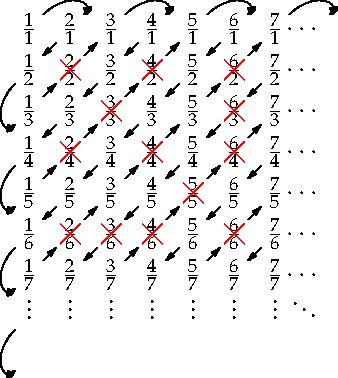
\includegraphics{intro-qcount}
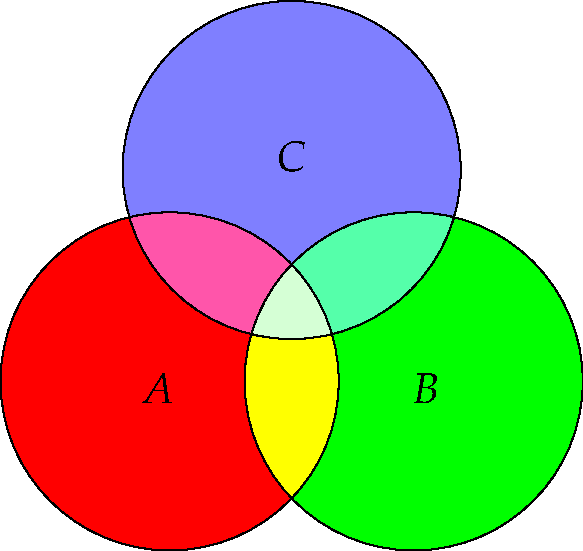
\includegraphics{intro-venndist}
\end{center}

\vfill\vfill\vfill

\clearpage


\pagenumbering{roman}


%\thispagestyle{empty}
\tableofcontents

\clearpage

\section*{Preface: What is Math 13 and who is it for?}
\label{sec:preface}
\addcontentsline{toc}{section}{\nameref{sec:preface}}

Math 13 was created by the late Howard Tucker, who chose the number as a joke and to position the class near the end of lower-division. Around 2012, program restructuring positioned Math 13 as the transition class between lower- and upper-division mathematics, introducing students to abstraction and proof, and serving as the key pre-requisite for upper-division pure courses.\smallbreak

The typical student is simultaneously working through lower-division calculus and linear algebra. Knowledge of such material is unnecessary and students are encouraged to take the class early so as to ease the transition from algorithmic to abstract mathematics and so that a proof-mentality may be brought to other lower-division classes.\smallbreak

This text evolved from the course notes dating back to 2008. Math 13 is something of a hydra due to the niche it occupies in UCI's program: part proof-writing, part discrete mathematics, and part introduction to specific upper-division topics. Logic is covered only at a basic level so that mathematical proofs may be engaged with as early as possible. Set theory is spread through the text; the intent is for dry `grammar' topics to be absorbed via engagement with more accessible and fun ideas. By the end of the course, interested students should be prepared for a formal study of logic and set theory at the upper-division level.


\boldsubsubsection{Learning Outcomes}

\begin{enumerate}
	\item Developing the skills necessary to read and practice abstract mathematics.
	\item Understanding the concept of proof and becoming acquainted with multiple proof techniques.
	\item Learning what sort of questions mathematicians ask and what excites them.
	\item Introducing upper-division mathematics by providing a taste of what is covered in several courses. For instance:
	\begin{description}
		\item[\normalfont\emph{Number Theory \& Abstract Algebra}] How can we perform arithmetic with remainders? Can you figure out what on which \emph{day} of the week you were born? 
		\item[\normalfont\emph{Geometry and Topology}] How can we visualize and work with objects such as the Möbius strip? How can we use sequences of sets to produce objects (fractals) that appear similar at all scales?
		\item[\normalfont\emph{To Infinity and Beyond!}] Why are some infinities greater than others?
	\end{description}
\end{enumerate}


\boldinline{Useful Texts}

The following texts are recommended if you want more exercises and material. The first two are available free online, while the remainder were previous textbooks for Math 13.

\begin{itemize}%\itemsep0pt
	\item \href{http://www.people.vcu.edu/~rhammack/BookOfProof/}{\emph{Book of Proof}}, Richard Hammack%, %2nd ed 
		%2013.
	
	\item \href{http://scholarworks.gvsu.edu/books/9/}{\emph{Mathematical Reasoning}}, Ted Sundstrom%, %2nd ed 
		%2014.

	\item \emph{Mathematical Proofs: A Transition to Advanced Mathematics}, Chartrand/Polimeni/Zhang%, %3\rd{} Ed
		%2013.%, Pearson.
	\item \emph{The Elements of Advanced Mathematics}, Steven G. Krantz%, %2\nd{} ed 
		%2002.%, Chapman \& Hall.
	\item \emph{Foundations of Higher Mathematics}, Peter Fletcher and C.~Wayne Patty%, %3\rd{} ed
		%2000.%, Brooks--Cole.
\end{itemize}




\clearpage

\iffalse

\subsection*{Notation}
\label{sec:notation}
\addcontentsline{toc}{section}{\nameref{sec:notation}}

Sets of numbers: $\N$, $\N_0$, $\Q$, $\R$


\clearpage

\fi

\pagenumbering{arabic}

\section{Introduction: What is a Proof?}\label{chap:intro}


The essential concept in higher-level mathematics is that of \emph{proof.} A basic dictionary entry might cover two meanings:
\begin{enumerate}%\itemsep0pt
	\item A test or trial of an assertion.
	\item An argument that establishes the validity (truth) of an assertion.
\end{enumerate}
In science and the wider culture, the first meaning predominates: a defendant was \emph{proved} guilty in court; a skin cream is clinically \emph{proven} to make you look younger; an experiment \emph{proves} that the gravitational constant is $9.81\mathrm{ms}^{-2}$. A common mistake is to assume that a \emph{proved assertion} is actually \emph{true.} Two juries might disagree as to whether a defendant is guilty, and for many crimes the truth is uncertain hence the more nuanced legal expression \emph{proved beyond reasonable doubt.}\smallbreak

In mathematics we use the second meaning: a proof establishes the incontrovertible \emph{truth} of some assertion. To see what we mean, consider a simple claim (mathematicians use the word \emph{theorem}).

\begin{thm}{}{sumeven}
	The sum of any pair of even integers is even.
\end{thm}

Hopefully you believe this statement. But how do we \emph{prove} it? We can \emph{test} it by verifying examples ($4+6=10$ is even, $(-8)+30=22$ is even, etc.), but we cannot expect to verify \emph{all} pairs this way. For a mathematical proof, we somehow need to test all possible examples simultaneously. To do this, it is essential that we have a clear idea of what is meant by an \emph{even integer.}

\begin{defn}{}{even}
	An integer is \emph{even} if it may be written in the form $2k$ where $k$ is an integer.
\end{defn}

\begin{proof}
	Let $x$ and $y$ be even. Then $x=2k$ and $y=2l$ for some integers $k$ and $l$. But then
	\[x+y=2k+2l=2(k+l)\tag{$\ast$}\]
	is even.
\end{proof}

The box \smash{\raisebox{8pt}{$\qedsymbol$}} indicates that we've finished our argument. Traditionally the letters Q.E.D.{} were used, an acronym for the Latin \emph{quod erat demonstrandum} (\emph{which is what was to be demonstrated}).\smallbreak

Consider how the proof depends crucially on the definition.

\begin{itemize}\itemsep0pt
	\item The theorem did not mention any \emph{variables,} though these were essential to the proof. The variables $k$ and $l$ come for free \emph{once you write the definition of evenness!} This is very common; a proof is often little more than rearranged definitions.
	\item According to the definition, $2k$ and $2l$ together represent \emph{all possible pairs} of even integers. It is essential that $k$ and $l$ be \emph{different symbols,} otherwise all you would be proving is that twice an even number is even!
	\item The calculation ($\ast$) is the easy bit; without the surrounding sentences and the direct reference to the definition of evenness, the calculation means nothing.
\end{itemize}

There is some sleight of hand here; a mathematical proof establishes truth only by reference to one or more definitions. In this case, the definition and theorem also depend on the meanings of \emph{integer} and \emph{sum,} but we haven't rigorously defined either since to do so would take us too far afield. In any context, some concepts will be considered too basic to merit definition.


\goodbreak


\boldsubsection{Theorems \& Conjectures}

Theorems are true mathematical statements that we can prove. Some are important enough to be named (the Pythagorean theorem, the fundamental theorem of calculus, the rank--nullity theorem, etc.), but most are simple statements such as Theorem \ref{thm:sumeven}.\smallbreak

In practice we are often confronted with \emph{conjectures}: statements we suspect to be true, but which we don't (yet) know how to prove. Much of the fun and messy creativity of mathematics lies in formulating and attempting to prove (or disprove) conjectures.\smallbreak

A conjecture is the mathematician's equivalent to the scientist's hypothesis: a statement one would like to be true. The difference in approach takes us right back to the dual meaning of \emph{proof.} The scientist \emph{tests} their hypothesis using the scientific method, conducting experiments which attempt (and hopefully fail!) to show that the hypothesis is incorrect. The mathematician tries to \emph{prove} that a conjecture is undeniably true by relying on logic. The job of a mathematical researcher is to formulate conjectures, prove them, and publish the resulting theorems. Creativity lies as much in the formulation as in the proof. Attempting to formulate your own conjectures is an essential part of learning mathematics; many will likely be false, but you'll learn a lot in the process!\medbreak

Here are two conjectures to give us a taste of this process.

\begin{conj}{}{n^2-1}
	If $n$ is any odd integer, then $n^2-1$ is a multiple of 8.
\end{conj}

\begin{conj}{}{n^2+n+41}
	If $n$ is any positive integer, then $n^2+n+41$ is prime.\footnotemark
\end{conj}

\footnotetext{\label{fn:introprime}A positive integer is \emph{prime} if it cannot be written as the product of two integers, both greater than one.}

How can we decide if these conjectures are true or false? To get a feel for things, we start by computing with several small integers $n$. In practice, this process is likely what lead to the formulation of the conjectures in the first place!
\[
	\def\arraystretch{1.2}
	\begin{array}{l||c|c|c|c|c|c|c}
		n & 1 & 3 & 5 & 7 & 9 & 11 & 13\\\hline
		n^2-1 & 0 & 8 & 24 & 48 & 80 & 120 & 168
	\end{array}
	\qquad\quad
	\begin{array}{l||c|c|c|c|c|c|c}
		n & 1 & 2 & 3 & 4 & 5 & 6 & 7\\\hline
		n^2+n+41 & 43 & 47 & 53 & 61 & 71 & 83 & 97
	\end{array}
\]
Since 0, 8, 24, 48, 80, 120 and 168 are all multiples of 8, and 43, 47, 53, 61, 71, 83 and 97 are all prime, both conjectures \emph{appear} to be true. Would you bet \$100 that this is indeed the case? Is $n^2-1$ a multiple of 8 \emph{for every} odd integer $n$? Is $n^2+n+41$ prime \emph{for every} positive integer $n$? Establishing whether each conjecture is true or false requires one of the following:

\begin{quote}
\begin{description}
  \item[\normalfont\emph{Prove it}] by showing it must be true in \underline{all} cases, or,
  \item[\normalfont\emph{Disprove it}] by finding \underline{at least one} instance in which the statement is false.
\end{description}
\end{quote}

Let us start with Conjecture \ref{conj:n^2-1}. If $n$ is an odd integer, then, by definition, we may write $n=2k+1$ for some integer $k$. Now compute the object of interest:
\[
	n^2-1 =(2k+1)^2-1 =(4k^2+4k+1)-1 =4k^2+4k =4k(k+1)
\]
We need to investigate whether this is \emph{always} a multiple of 8. Since $k$ is an integer, $n^2-1$ is plainly a multiple of 4, so everything comes down to deciding whether $k(k+1)$ is \emph{always even.} Do we believe this? We return to testing some small values of $k$:
\[
	\def\arraystretch{1.2}
	\begin{array}{l||c|c|c|c|c|c|c}
		k & -2 & -1 & 0 & 1 & 2 & 3 & 4\\\hline
		k^2+k & 2 & 0 & 0 & 2 & 6 & 12 & 20
	\end{array}
\]
Once again, the claim seems to be true for small values of $k$, but how do we know it is true for \emph{all} $k$? Again, the only way is to \emph{prove} or \emph{disprove it}. Observe that $k(k+1)$ is the \emph{product of two consecutive integers.} This is great, because for any two consecutive integers, one is even and the other odd, so their product must be even. Conjecture \ref{conj:n^2-1} is indeed a \emph{theorem!}\smallbreak

Everything so far has been investigative. Scratch work is an essential part of the process, but it isn't something we should expect a reader to have to fight their way through. We therefore offer a formal proof. This is the final result of our deliberations; investigate, spot a pattern, conjecture, prove, and finally present our work in as clean and convincing a manner as we can.

\begin{thm}{}{n^2-1}
	If $n$ is any odd integer, then $n^2-1$ is a multiple of 8.
\end{thm}

\begin{proof}
	Let $n$ be any odd integer. By definition, we may write $n=2k+1$ for some integer $k$. Then
	\[
		n^2-1=(2k+1)^2-1=(4k^2+4k+1)-1=4k^2+4k=4k(k+1)
	\]
	We distinguish two cases. If $k$ is even, then $k(k+1)$ is even and so $4k(k+1)$ is divisible by 8.\smallbreak
	If $k$ is odd, then $k+1$ is even. Therefore $k(k+1)$ is again even and $4k(k+1)$ divisible by 8.\smallbreak
	In both cases $n^2-1=4k(k+1)$ is divisible by 8.
\end{proof}

All that work, just for five lines of clean argument! But wasn't it \emph{fun}?\medbreak

When constructing elementary proofs it is common to feel unsure over how much detail to supply. We plainly relied on the definition of \emph{oddness,} but we also used the fact that a product is even whenever either factor is even; does this need a proof? Since the purpose of a proof is to convince the reader, the appropriateness of an argument will depend on context and your audience: if you are trying to convince a middle-school student, maybe you should justify this step more fully, though the cost would be a longer argument that might be harder to grasp in its totality. A perfect proof that is best for all situations is unlikely to exist! A good rule is to imagine you are writing for another mathematician at the same level as yourself---if a fellow student believes your argument, that's a good sign of its validity.
\bigbreak

Now consider Conjecture \ref{conj:n^2+n+41}. The question is whether $n^2+n+41$ is prime for \emph{every} positive integer $n$. When $n\le 7$ the answer is yes, but examples do not make a proof! To investigate further, return to the definition of prime (Footnote \ref{fn:introprime}): is there a positive integer $n$ for which is $n^2+n+41$ can be factored as a product of two integers, both at least 2? A straightforward answer is staring us in the face! When $n=41$ such a factorization certainly exists:
\[
	n^2+n+41 =41^2+41+41 =41(41+1+1) =41\cdot 43
\]
We call $n=41$ a \emph{counterexample}; it shows that there is at least one integer $n$ for which $n^2+n+41$ is \emph{not} prime. Conjecture \ref{conj:n^2+n+41} is therefore false (it has been \emph{disproved}).



\boldsubsubsection{Planning and Writing Proofs}
\phantomsection\label{sec:proofplan}

Your main responsibility in this course is the construction of proofs. Their sheer variety means that, unlike in elementary calculus, you cannot simply practice computing tens of similar problems until the process becomes automatic. So how do you learn to write proofs?\smallbreak

The first step is to \emph{read} other arguments. Don't just accept them, make sure you \emph{believe} them: check the calculations, verify claims, rewrite the argument in your own words adding any clarification you think necessary.\smallbreak

As you read others' arguments, the question will often arise: \emph{how did they ever come up with this?} As our work on Theorem \ref{thm:n^2-1} shows, the source of a proof is often less magical than it appears; usually the author experimented until they found something that worked. Most of that experimentation gets hidden in the final proof which should be as clean and easy to read as possible. Imagine it as a concert performance after lots of private practice; no-one wants to hear wrong notes at the Carnegie Hall!\smallbreak

In order to bridge the gap, we recommend splitting the proof-writing process into several steps.

\begin{description}
	\item[Interpret] Make sense of the statement. What is it saying? Can you rephrase in a way that is clearer to you? What are you assuming? The most important part of this step is identifying the \emph{logical structure} of the statement. We'll discuss this at length in the next chapter.
    
	\item[Brainstorm] Convince \emph{yourself} that the statement is true. First, look up the relevant definitions. Next, think of some instances where the conditions of the statement are met. Try out some examples, and ask yourself what makes the claim work in those instances. Examples can be crucial for building intuition about \emph{why} the claim is true and can sometimes suggest a proof strategy. Review other theorems that relate to these definitions. Do you know any theorems that relate your assumptions to the conclusion? Have you seen a proof of a similar statement before?

	\item[Sketch] Build the skeleton of your proof. Think again about what you are assuming and what you are are you trying to prove. As we'll see in the next chapter, it is often straightforward to write down reasonable \emph{first} and \emph{last} steps (the bread slices of a \emph{proof-sandwich}). Try to connect these with informal arguments. If you get stuck, try a different approach.\par
	This step is often the longest in the proof-writing process. It is also where you will be doing most of your calculations. You can be as messy as you want because \emph{no-one ever has to see it}! Once you've learned a variety of different proof methods, this is a good stage at which to experiment with different approaches.
  
	\item[Prove] Once you have a suitable sketch, it's time to prove the statement to the world. Translate your sketch into a linear story, written in complete sentences. Carefully word your explanations and avoid shorthand, though well-understood mathematical symbols like $\Longrightarrow$ are encouraged. The result should be a clear, formal proof like you'd find in a mathematics textbook. Although you are providing a mathematical argument, your proof should read like prose. 

	\item[Review] Finally, \emph{review} your proof. Assume the reader is meeting the problem for the first time and has not seen your sketch. Read your proof with skepticism; consider its readability and flow. Get read of unnecessary claims and revise the wording if necessary. Read your proof out loud. If you're adding extra words that aren't written down, include them in the proof. Finally, share your work with others. Do they understand it \emph{without any additional input from you}?
\end{description}

\goodbreak



\boldsubsubsection{Conjectures: \emph{True} or \emph{False}?}

Higher-level mathematics is all about the important links between proofs, definitions, theorems and conjectures. We prove theorems (and solve homework problems) because they make us use, and aid our understanding of, definitions. We state definitions to help us formulate conjectures and prove theorems. One does not \emph{know} mathematics, one \emph{does} it. Mathematics is a \emph{practice}; an art as much as it is a science.\medbreak

With this in mind, do your best to prove or disprove the following conjectures. Don't worry if you're currently unsure as to the meanings of some of the terms or notation: ask! It will all be covered formally soon enough. At the end of the course, revisit these problems to realize how much your proof skills have improved. 

\begin{enumerate}
	\item The sum of any three consecutive integers is even.
	\item There exist integers $m$ and $n$ such that $7m+5n =4$.
	\item Every common multiple of 6 and 10 is divisible by 60.
	\item There exist integers $x$ and $y$ such that $6x+9y =10$.
	\item For every positive real number $x$, $x+\frac{1}{x} $ is greater than or equal to 2.
	\item If $x$ is any real number, then $x^2\ge x$.
	\item If $n$ is any integer, $n^2+5n$ must be even.
	\item If $x$ is any real number, then $|x|\ge -x$.
	\item If $n$ is an integer greater than 2, then $n^2-1$ is not prime.
	\item An integer is divisible by 5 when its last digit is 5.
	\item If $r$ is a rational number, then there is a non-zero integer $n$ for which $rn$ is an integer.
	\item There is a smallest positive real number.
	\item For all real numbers $x$, there exists a real number $y$ for which $x<y$.
	\item There exists a real number $x$ such that, for all real numbers $y$, $x<y$.
	\item The sets $A=\{n\in\N:n^2<25\}$ and $B=\{n^2:n\in\N\text{ and }n<5\}$ are equal. Here $\N$ denotes the set of natural numbers.
\end{enumerate}



